\scanpage{19}
\margin{\figure{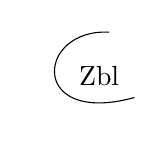
\begin{tikzpicture}\node (z) at (0,0){\unsure{Zbl}};\draw (.45,-.28) .. controls (-.9,-.65) and (-.8,.6) .. (.13,.55);\end{tikzpicture}}}
\inserted{d'où $S(t)\unsure{-|\longrightarrow}S(s)$.}
On va définir un \unsure{hom|isom} $\unsure{A(s)}\simeq B\times_{\deleted{\unsure{V}}S}\unsure{S(s)}$, tel que par \unsure{chgt de base} $S(t)\longrightarrow S(s)$, on retrouve l'isom $A(t)\simeq B\times_S S(t)$ donné. \deleted{Un tel \unsure{isom}}

\uline{Lemme} $S$ schéma \unsure{noethérien|noeth.}, \inserted{\deleted{[excellent]}} $t\in S$, $B$ schéma abélien sur $S$. Alors $\exists$ voisinage ouvert $V$ de $t$, \deleted{\unsure{avec} \unsure{les} \unsure{comp.} \unsure{de} \inserted{\deleted{\unsure{irréduc.}}}} tel que pour \deleted{$\unsure{\Rightarrow}\ \forall s\in V$,} tout voisinage ouvert $\unsure{W'|V'}$ de $t$, $V'\subset V$, tout schéma abélien $B'$ sur $V'$, et tout isom $\varphi_0:B'\times_S\operatorname{Spec}O_{S,t}\simeq B\times_S\operatorname{Spec}\underline O_{S,t}$, $\varphi_0$ se prolonge (de façon unique en un isom $\varphi:B'\simeq B|V'$.

L'unicité sera garantie dès que \unsure{toute composante} \unsure{ponctuelle|point associé} de $V$ rencontre $t$, i.e. que $V$ est contenu dans \unsure{la réunion|le complément} des comp. irréduc. de $S$ ne contenant pas $t$.

\deleted{Soit $S'\longrightarrow S$}
On peut supposer $S$ affine. \inserted{Supposons d'abord $S$ excellent.} Soit $S'\longrightarrow S$ fini, tel que $S'\times_S S(s)\longrightarrow S(s)$ soit birationnel, et $S'$ réduit et géom. unibr.

Alors
\mspage{18}
